\documentclass[uplatex,dvipdfmx,a4paper,11pt]{jsarticle}

\usepackage[top=25mm,bottom=25mm,left=25mm,right=25mm]{geometry}
\usepackage{array}
\usepackage{tabularx}
\usepackage{booktabs}
\usepackage{enumitem}
\usepackage{graphicx}

\setlength{\parindent}{0pt}
\setlength{\parskip}{0.6em}

\usepackage{titlesec}
\titleformat{\section}
  {\normalfont\Large\bfseries}{\thesection.}{0.6em}{}
\titleformat{\subsection}
  {\normalfont\large\bfseries}{\thesubsection}{0.6em}{}
\titlespacing*{\section}{0pt}{1.2em}{0.6em}
\titlespacing*{\subsection}{0pt}{1.0em}{0.4em}

\newcommand{\sectionrule}{\par\medskip\noindent\rule{\linewidth}{0.6pt}\par\medskip}

\renewcommand{\labelitemi}{\textbullet}
\renewcommand{\labelitemii}{\textopenbullet}
\setlist[itemize]{leftmargin=1.6em,itemsep=0.1em,topsep=0.2em}
\setlist[enumerate]{leftmargin=2.0em,itemsep=0.1em,topsep=0.2em}

\providecommand{\textopenbullet}{\ensuremath{\circ}}

\begin{document}

{\LARGE\bfseries 作業ログ}\par\bigskip

報告者：梅澤颯太

報告日：2026年6月23日

プロジェクト名：タクトーン～IMU ジェスチャーで奏でるArduino オーケストラ～

\sectionrule

\section{進捗サマリー（要約）}

\begin{itemize}
  \item 全体進捗率：95\%
  \item マイルストーン達成状況：ガントチャートに載っている個人のタスクは全て完了
  \item 主要成果：
    \begin{itemize}
      \item 指揮棒側の3Dプリンタ出力に向けて，基本形状を作成した．
      \item 部品を収めるための寸法と外形を調整し，出力前の試作モデルを完成させた．
    \end{itemize}
  \item 課題：
    \begin{itemize}
      \item 試作モデルは未出力であり，実物での寸法，部品の収まり，持ちやすさを確認する必要がある．
      \item 3Dプリンタ出力後に問題が見つかった場合は，配線の逃げや固定方法を含めてモデルを修正する必要がある．
    \end{itemize}
\end{itemize}

\subsection{ガントチャート}

\begin{figure}[htbp]
  \centering
  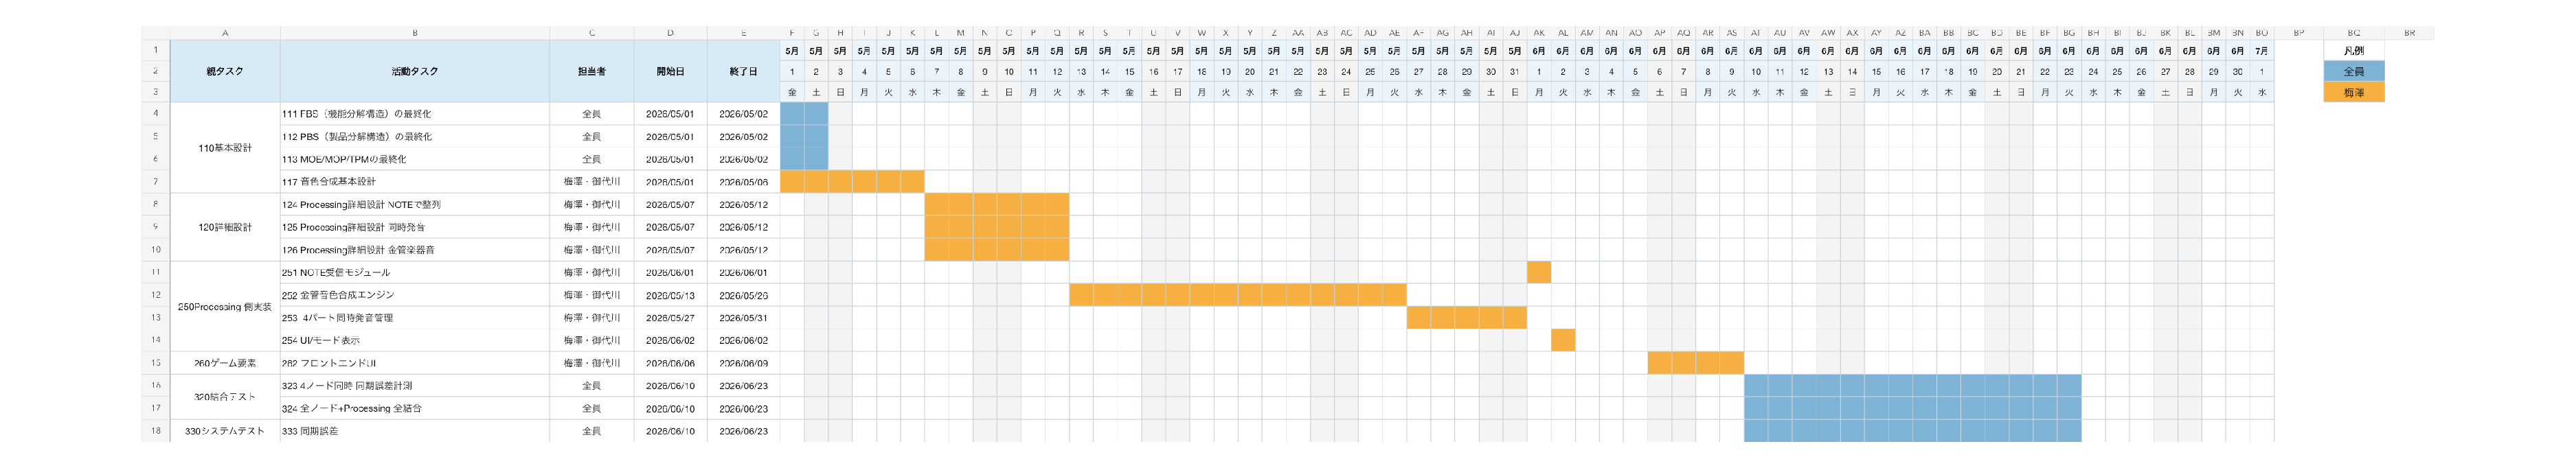
\includegraphics[width=\linewidth]{fig/ガントチャート_梅澤_全員.pdf}
  \caption{全体のガントチャート}
\end{figure}

\sectionrule

\section{作業ログ（詳細トラッキング）}

\begin{tabularx}{\linewidth}{@{}p{0.16\linewidth}p{0.12\linewidth}XX@{}}
\toprule
日付 & 作業時間 & 作業内容 & 成果・メモ \\
\midrule
2026/06/21 & 1.5h & 指揮棒側の3Dモデルの基本形状を作成した． & 前回のモデリング練習をもとに，指揮棒として使用する外装の基本形状を作成し，部品を収める位置と全体の大きさを検討した． \\
2026/06/23 & 1h & 3Dモデルの寸法と形状を調整した． & 部品の収まりと持ちやすさを考慮して寸法と外形を調整し，3Dプリンタで出力する前段階の試作モデルを完成させた． \\
\bottomrule
\end{tabularx}

\sectionrule

%================================================================
% 3. 課題管理
%================================================================
\section{課題管理}

\begin{tabularx}{\linewidth}{@{}p{0.20\linewidth}Xp{0.08\linewidth}p{0.08\linewidth}Xp{0.11\linewidth}p{0.09\linewidth}@{}}
\toprule
課題 & 発生原因 & 影響度 & 優先度 & 対策 & 期限 & 状態 \\
\midrule
試作モデルの出力確認 & 現時点では3Dモデル上での確認のみで，3Dプリンタによる出力を行っていない． & 高 & 高 & 試作モデルを出力し，寸法，強度，部品の収まりを確認する． & 次回作業時 & 対応予定 \\
持ちやすさと配線スペースの確認 & 画面上では実際に握ったときの感覚や，配線を通した際の余裕を確認できない． & 中 & 中 & 出力した試作品へ部品を仮配置し，持ちやすさと配線の逃げを確認して必要箇所を修正する． & 実機組立前 & 対応予定 \\
\bottomrule
\end{tabularx}

\sectionrule

%================================================================
% 4. AI利用状況と検証
%================================================================
\section{AI利用状況と検証（再現性重視）}

\subsection{利用内容}

\begin{itemize}
  \item 利用目的：作業ログ文章の作成補助
  \item 入力（プロンプト要旨）：
    \begin{itemize}
      \item 前週の作業ログを参考に，同じ構成で今週分の作業ログを作成するよう依頼した．
      \item 6月21日に1時間30分かけて指揮棒の基本形状を作成し，6月23日に1時間かけて寸法と形状を調整して試作モデルを完成させたことを伝えた．
    \end{itemize}
  \item 出力概要：
    \begin{itemize}
      \item 前週の形式に合わせて，進捗サマリー，作業ログ，課題管理，AI利用状況，次回計画の文章を作成した．
      \item 3Dモデルの作成段階と，出力後に確認すべき課題を分けて整理できた．
    \end{itemize}
\end{itemize}

\sectionrule

\subsection{検証方法}

\begin{itemize}
  \item 検証手法：
    \begin{itemize}
      \item 作業ログに記載された日付，作業時間，作業内容が実際の作業と一致しているかを確認する．
      \item 試作モデルを実物として完成したものと誤解させる表現がないかを確認する．
    \end{itemize}
  \item 検証手順：
    \begin{enumerate}
      \item 6月21日と6月23日の作業内容を生成された文章と照らし合わせる．
      \item 作業時間の合計が2時間30分であることを確認する．
      \item 成果が3Dプリンタ出力前の試作モデルであることを確認する．
    \end{enumerate}
\end{itemize}

\sectionrule

\subsection{ファクトチェック結果}

\begin{itemize}
  \item 一致点：
    \begin{itemize}
      \item 日付，作業時間，基本形状の作成，寸法と形状の調整，試作モデルの完成について，実際の作業内容と一致していた．
    \end{itemize}
  \item 不一致・疑義：
    \begin{itemize}
      \item なし
    \end{itemize}
  \item 最終判断：
    \begin{itemize}
      \item レポート本文として採用する．
    \end{itemize}
  \item 根拠：
    \begin{itemize}
      \item 実際の作業内容と作業時間を正確に反映し，未実施の3Dプリンタ出力を次回課題として区別しているため．
    \end{itemize}
\end{itemize}

\sectionrule

%================================================================
% 5. 次回計画
%================================================================
\enlargethispage{2\baselineskip}
\section{次回計画}

\begin{itemize}
  \item 目標：
    \begin{itemize}
      \item 完成した試作モデルを3Dプリンタで出力する．
      \item 出力した試作品に電子部品を配置し，寸法と持ちやすさを確認する．
    \end{itemize}
  \item 達成基準：
    \begin{itemize}
      \item 3Dプリンタでモデルを正常に出力できること．
      \item 電子部品と配線を収められ，指揮棒として無理なく持てる形状であること．
      \item 問題が見つかった場合に，修正箇所を具体的に整理できること．
    \end{itemize}
  \item 期限：
    \begin{itemize}
      \item 次回作業時
    \end{itemize}
\end{itemize}

\sectionrule

%================================================================
% 6. その他
%================================================================
\section{その他}

\begin{itemize}
  \item 今週は前週に行ったモデリング練習をもとに，実際の指揮棒用試作モデルを作成した．
  \item 3Dプリンタ出力後は，モデル上の寸法だけでなく，部品の固定，配線の取り回し，握ったときの安定性を確認する必要がある．
\end{itemize}

\sectionrule

%================================================================
% 7. 付録
%================================================================
\section{付録}

無し

\sectionrule

\end{document}
